\documentclass[]{article}
\usepackage{lmodern}
\usepackage{amssymb,amsmath}
\usepackage{ifxetex,ifluatex}
\usepackage{fixltx2e} % provides \textsubscript
\ifnum 0\ifxetex 1\fi\ifluatex 1\fi=0 % if pdftex
  \usepackage[T1]{fontenc}
  \usepackage[utf8]{inputenc}
\else % if luatex or xelatex
  \ifxetex
    \usepackage{mathspec}
  \else
    \usepackage{fontspec}
  \fi
  \defaultfontfeatures{Ligatures=TeX,Scale=MatchLowercase}
\fi
% use upquote if available, for straight quotes in verbatim environments
\IfFileExists{upquote.sty}{\usepackage{upquote}}{}
% use microtype if available
\IfFileExists{microtype.sty}{%
\usepackage[]{microtype}
\UseMicrotypeSet[protrusion]{basicmath} % disable protrusion for tt fonts
}{}
\PassOptionsToPackage{hyphens}{url} % url is loaded by hyperref
\usepackage[unicode=true]{hyperref}
\hypersetup{
            pdfborder={0 0 0},
            breaklinks=true}
\urlstyle{same}  % don't use monospace font for urls
\usepackage{graphicx,grffile}
\makeatletter
\def\maxwidth{\ifdim\Gin@nat@width>\linewidth\linewidth\else\Gin@nat@width\fi}
\def\maxheight{\ifdim\Gin@nat@height>\textheight\textheight\else\Gin@nat@height\fi}
\makeatother
% Scale images if necessary, so that they will not overflow the page
% margins by default, and it is still possible to overwrite the defaults
% using explicit options in \includegraphics[width, height, ...]{}
\setkeys{Gin}{width=\maxwidth,height=\maxheight,keepaspectratio}
\IfFileExists{parskip.sty}{%
\usepackage{parskip}
}{% else
\setlength{\parindent}{0pt}
\setlength{\parskip}{6pt plus 2pt minus 1pt}
}
\setlength{\emergencystretch}{3em}  % prevent overfull lines
\providecommand{\tightlist}{%
  \setlength{\itemsep}{0pt}\setlength{\parskip}{0pt}}
\setcounter{secnumdepth}{0}
% Redefines (sub)paragraphs to behave more like sections
\ifx\paragraph\undefined\else
\let\oldparagraph\paragraph
\renewcommand{\paragraph}[1]{\oldparagraph{#1}\mbox{}}
\fi
\ifx\subparagraph\undefined\else
\let\oldsubparagraph\subparagraph
\renewcommand{\subparagraph}[1]{\oldsubparagraph{#1}\mbox{}}
\fi

% set default figure placement to htbp
\makeatletter
\def\fps@figure{htbp}
\makeatother


\date{}

\begin{document}

\tableofcontents

\newpage
\section{Introduction}\label{introduction}

\subsection{Infrastructure as code}\label{infrastructure-as-code}

L'infrastructure as code ou encore ``infrastructure programmable'' est
un type d'infrastructure IT administré via du code (avec divers langage
possible suivant la technologie utilisée). L'IAC est utilsée à la fois
pour gérer les configurations, déployer et automatiser le
provisionnement d'une infrastructure. Nous allons donc avoir le code
écrit pour pouvoir fournir et gérer nos serveurs tout en permettant
d'automatiser les tâches. L'IAC, n'est plus seulement utilisée par les
admins sys, en effet les développeurs de logiciels et d'applications
peuvent facilement écrire un code d'infrastructure pour pouvoir se créer
un environnement à des fins expérimentales pour tester leurs logiciels.
De nombreux outils utilisent l'IAC comme par exemple Vagrant qui va
permettre de créer un environnement virtuel grâce au code contenu dans
le Vagrantfile, ou encore Ansible qui va lui permettre un
provisionement. Plus récemment le logiciel Docker qui permet
d'automatiser le déploiement d'applications dans des conteneurs
logiciels utilise également l'IAC avec les dockerfile. Une
infrastructure as code à aussi la particularité de pouvoir être déployée
(suivant la technologie que l'on utlise) à la fois sur des machines
locales, des serveurs, des environnements virtuels ou encore dans le
cloud. L'IAC permet aussi de suivre les modifications d'une
infrastructure, en cas de problème il sera alors très simple de revenir
à la configuration précédente. Cependant, l'infrastructure as code
possède aussi des inconvénients. Une mauvaise configuration sera
dupliquée sur toutes les machines concernées, il faut aussi faire
attention aux modifications que l'on fait, par exemple si on modifie la
configuration d'un serveur manuellement, elle n'aura plus rien à voir
avec le modèle de base qui est dans le code. L'IAC utilisant de nombreux
logiciels différents, il faut aussi effectuer des tâches de recherche
pour savoir lequel va le plus correspondre à ses besoins.

\subsection{Mouvance Devops}\label{mouvance-devops}

Devops est la concaténation du mot \emph{development} et
\emph{operations} (en anglais). Au début de l'informatique en
entreprise, les applications ne jouaient pas un grand rôle et étaient
peu intégrées, il n'y avait alors pas de séparation entre développement
et opérations, la même équipe d'informaticiens se chargeait à la fois du
développement de l'application et de sa maintenance.

L'évolution de l'informatique d'entreprise a fait que les logiciels ont
évolués et prisent plus de place en terme d'utilisation ce qui a conduit
à une séparation de dev et ops en deux équipes distinctes. L'équipe de
dev apportait les changements au logiciels souvent le plus rapidement
possible pour un moindre coût tandis que l'équipe ops garantissait la
stabilité du système en ce concentrant sur la qualité.

\begin{quote}
Sanjeev Sharma et Bernie Coyne7 recommandent :
\end{quote}

\begin{verbatim}
un déploiement régulier des applications, la seule répétition contribuant à fiabiliser le processus ;
un décalage des tests "vers la gauche", autrement dit de tester au plus tôt ;
une pratique des tests dans un environnement similaire à celui de production ;
une intégration continue incluant des "tests continus" ;
une boucle d'amélioration courte (i.e. un feed-back rapide des utilisateurs) ;
une surveillance étroite de l'exploitation et de la qualité de production factualisée par des métriques et indicateurs "clé".
\end{verbatim}

La mise en oeuvre du DevOPs vient de la vonlonté de travaller ensemble
pour produire de la valeur pour l'entreprise. Pour cela on va définir
des objectifs communs aux équipes de développement et de production

\subsection{Le cloud computing}\label{le-cloud-computing}

Le Cloud computing est un concept qui s'oppose à la notion de stockage
local. Pour faire simple, le cloud computing va permettre d'utiliser des
ressources informatiques sans les posséder réellement, de fournir des
services ou des applications accessibles partout depuis internet. Il y a
de nombreux avantages à utiliser un cloud computing. Tout d'abord,
l'utilisateur n'a pas d'infrastructure à gérer, ce qui est parfois plus
simple pour des entreprises, car c'est le fournisseur cloud qui s'occupe
de la maintenance de ses équipements. Il permet donc une réduction des
coûts en n'ayant pas besoin d'investir dans une infrastructure interne,
mais en payant uniquement ce qu'il consomme à son fournisseur de cloud.
Cependant, on a bien entendu des inconvénients comme le fait de savoir
où le prestataire de service stocke nos données (territoire national ou
pas -\textgreater{} problèmes de loi), la sécurité du cloud sur le
stockage, la confidentialité et aussi vis-à-vis des hackers, on doit
donc avoir confiance en le prestataire.

Il existe trois catégories de services pour le cloud computing.

\begin{itemize}
\item
  Le cloud privé : infrastructure pouvant être gérée en interne par
  l'entreprise ou par un prestataire qui se verra confier les tâches
  relatives à l'administration et l'optimisation des performances. Il
  est conçu uniquement pour un seul utilisateur pour répondre aux mieux
  aux besoins. Ce modèle a pour avantage de laisser à l'entreprise le
  contrôle à la fois sur la gestion des services, des données et de
  l'infrastructure. Le fait que ce soit un système fermé permet de mieux
  connaître les paramètres de sécurité, les garanties de service et la
  politique de confidentialité. Cependant, le déploiement de ce type
  d'infrastructure est très coûteux à mettre en place.
\item
  Le cloud public : structure souple et ouverte proposée par des tiers
  spécialisés comme Amazon Web Services, Microsoft Azure, IBM, Google
  Compute Engine ou encore Cloudwatt. Le plus souvent ces services sont
  vendus sur demande, le client va donc être facturé sur ce qu'il
  consomme. L'ensemble de l'infrastructure est géré par le fournisseur
  de service, ce qui permet une utilisation plus souple pour le client.
  Le cloud public s'adapte rapidement aux différents besoins, c'est ce
  qui charme le plus les entreprises (ne pas être limités par le volume
  de données). L'un des inconvénients est l'absence de contrôle sur
  cette solution, que ce soit sur les données, sur la rapidité (beaucoup
  d'utilisateurs serveur mutualisé) pas forcément adapté à nos besoins.
  Si l'entreprise recherche de la confidentialité, le service de cloud
  public n'est pas recommandé. Pour l'aspect économique, ce service va
  permettre une réelle économie, car il n'y a pas de matériel ou
  d'informaticien à gérer, mais plus le client utilisera le service plus
  la facture sera élevée.
\item
  le cloud hybride : est un système mixte qui mélange le cloud privé et
  public. Le client va faire appel à plusieurs clouds indépendants les
  uns des autres, ce qui permet de placer les données sensibles et
  confidentielles dans un cloud privé et les autres dans un cloud
  public. Avec ce type de cloud, on va aussi pouvoir réduire les coûts
  d'exploitation en tirant l'avantage des deux infrastructures, on va
  ainsi dimensionner son cloud privé pour une charge moyenne et le cloud
  public pour répondre aux montées de charge.
\end{itemize}

(TODO : encore du C/c) Les différents modèles de cloud englobent
plusieurs types de services, que l'on peut regrouper en trois parties :
- IaaS - Infrastructure As a Service : le but est d'offrir un service de
bas niveau, le consommateur peut alors choisir le système d'exploitation
et y installer les outils adaptés à ses besoins. Il est possible de
louer dynamiquement des machines virtuelles pour une courte durée. Il
est également possible de louer un ensemble de machines constituant une
infrastructure externe. Les acteurs français du IaaS sont Online.net,
OVH (Kimsufi), \ldots{} - PaaS - Platform As a Service : cette fois-ci,
le système est déjà installé, c'est le fournisseur qui gère le système
et l'infrastructure. Le consommateur profite alors de la plate-forme
pour y installer les applications souhaitées. Un exemple illustrant bien
le PaaS est l'hébergement web, où l'hébergeur fournit une plate-forme
souvent LAMP4, afin d'y héberger des sites web ou des systèmes de
gestion de contenus. - SaaS - Software As a Service : c'est une suite
d'applications proposées aux consommateurs. Ces derniers ne s'occupent
de rien, c'est le fournisseur qui gère l'intégralité de
l'infrastructure, des systèmes et des logiciels. Gmail, Office Web Apps,
Google Apps sont les fournisseurs de SaaS les plus connus.

\subsection{Contexte du projet}\label{contexte-du-projet}

Xilopix (NOTE : url du site) est une start-up basée à Epinal qui
développe un moteur de recherche pensée pour le tactile. Leur
technologie se diffère des autres navigateurs web, car lors d'une
recherche on va avoir une combinaison d'éléments de différentes natures
(textes, images, vidéos, pages web, géolocalisation, sons, etc.) qui
sera possible d'affiner en choisissant à quel info on souhaite avoir
accès. De fait Xilopix va permettre d'améliorer la pertinence des
résultats de recherche tout en offrant une nouvelle expérience
utilisateur à la fois visuelle, tactile et ludique. Xilopix utilise une
infrastructure cloud avec plusieurs hébergeurs (ovh et cloudwatt) tous
sur OpenStack. OpenStack permet de faire du IaaS (le consommateur peut
choisir pour ses machines le système d'exploitation et les différents
outils dont il a besoin), il va monter une infrastructure dans le
domaine du cloud computing. Cependant, Xilopix souhaiterait ne plus être
dépendant d'OpenStack et être libre d'utiliser AWS par exemple. C'est
dans cette optique qu'intervient Terraform.

\subsection{Enjeu et problématique}\label{enjeu-et-probluxe9matique}

L'objectif du projet est de développer un proof of concept sur l'outil
Terraform pour pouvoir démontrer les avantages de cet outil.

\begin{quote}
Un proof of concept est une réalisation expérimentale concrète et
préliminaire, courte ou incomplète, illustrant une certaine méthode ou
idée afin d'en démontrer la faisabilité. (NOTE source wikipédia:
https://fr.wikipedia.org/wiki/Preuve\_de\_concept)
\end{quote}

Pour se faire, nous allons mettre en place un cluster de quatres
machines virtuelles ainsi qu'un réseau, un sous-réseau et un routeur
pour recréer une infrastructure minimale fonctionnelle avec l'outil
Terraform. Xilopix ayant une infrastructure utilisant OpenStack, nous
avons créer des configurations fonctionnant pour OpenStack.

A partir de ces études, Xilopix pourra choisir d'utiliser ou non cet
outil.

La finalité du projet est d'obtenir une création rapide et demandant un
minimum d'intervention humaine pour déployer plusieurs machines aussi
bien sous OpenStack, sous AWS ou tout autre provider. Terraform va donc
nous permettre de réduire les dépendances entre ces outils et les
infrastructures qui les utilisent tout en facilitant la mise en place de
machines.

\subsection{Quelques mots sur
Openstack}\label{quelques-mots-sur-openstack}

OpenStack est un ensemble de logiciels/modules open source permettant de
déployer des infrastructures de cloud computing. La technologie possède
une architecture modulaire composée de plusieurs projets (Nova, Swift,
Glance\ldots{}) qui permettent de contrôler les différentes ressources
des machines virtuelles telles que la puissance de calcul, le stockage
ou encore le réseau inhérents au centre de données sollicité.

\subsection{Quelques mots sur
Terraform}\label{quelques-mots-sur-terraform}

Terraform est une solution pour la construction, la modification et le
versionning d'infrastructure de manière sûre et efficace. Développé
depuis 2013 par HashiCorp, c'est un outil en pleine expansion. Il permet
de gérer plusieurs fournisseurs de services existant ainsi que des
solutions développées en interne. Avec cette technologie, il est
possible d'administrer des composants de bas niveau comme les IaaS, le
stockage et la mise à niveau, ainsi que des composants haut niveau comme
les entrées DNS et les fonctionnalités SaaS.

\section{Openstack / python-nova}\label{openstack-python-nova}

Xilopix fonctionne avec Openstack, nous avons donc du apprendre
rapidement son fonctionnement pour pouvoir ensuite travailler plainement
sur sa mise en place avec Terraform.

\subsection{Introduction}\label{introduction-1}

Openstack est un projet qui est né en 2010 (licence Apache 2.0) par
l'entreprise RackSpace. OpenStack est un logiciel libre qui va nous
permettre de faire du cloud computing et qui permet de faire du IaaS
pour du cloud privé ou public. Le but d'Openstack est d'offrir à son
utilisateur une multitude de module qui va lui permettre de faire de
l'infrastructure as a service c'est à dire deployer des machines
virtuelles en optimisant les ressources materielles. On peut les
deployer dynamiquement pour une courte durée, mais il est également
possible de deployer un ensemble de machines constituant une
infrastructure externe.

\subsection{Les modules : services
d'OpenStack.}\label{les-modules-services-dopenstack.}

Openstack se compose de plusieurs modules pour fonctionner, avec des
modules plus ou moins important pour la création d'infrastructure.

\subsubsection{Keystone, le service
d'identité}\label{keystone-le-service-didentituxe9}

Fournit un service d'authentification et d'autorisation pour les autres
services d'OpenStack. Fournit un catalogue de endpoints pour tous les
services d'OpenStack.

\subsubsection{Glance, la gestion
d'images}\label{glance-la-gestion-dimages}

Stocke et récupère des images disques de machines virtuelles. OpenStack
Compute les utilise lors du provisioning d'instance.

\subsubsection{Nova, le Compute}\label{nova-le-compute}

Nova est le coeur du project Openstack, il gère le cycle de vie des
instances dans un environnement OpenStack. Les tâches incluent la
planification, la création et la mise hors service de machines
virtuelles à la demande.

\subsubsection{Horizon, l'interface web}\label{horizon-linterface-web}

Fournit un portail libre-service de type web permettant d'interagir avec
les services sous-jacents d'OpenStack, comme le lancement d'une
instance, l'attribution d'adresses IP ou la configuration des contrôles
d'accès.

\subsubsection{Cinder, le service de disques
persistants}\label{cinder-le-service-de-disques-persistants}

Fournit un stockage bloc persistant aux instances en cours d'exécution.
Son architecture basée sur des drivers de type plugin facilite la
création et la gestion des devices de stockage bloc.

\subsubsection{Neutron, la gestion de
réseaux}\label{neutron-la-gestion-de-ruxe9seaux}

Permet le Network-Connectivity-as-a-Service pour d'autres services
d'OpenStack, comme Compute. Il fournit une API utilisateur pour définir
les réseaux et les attachements à ces réseaux. Il possède une
architecture modulaire qui permet le support de la plupart des
fournisseurs et des technologies réseau.

\subsubsection{Swift, le stockage
d'objet}\label{swift-le-stockage-dobjet}

Stocke et récupère des objets de données non structurées via une API
RESTful basée sur HTTP. Le service est hautement tolérant aux pannes
avec sa réplication de données et son architecture de type scale-out.
Son implémentation diffère des serveurs de fichiers à répertoires
montables. Le service écrit les objets et les fichiers vers plusieurs
disques, en s'assurant que les données sont répliquées sur un cluster de
serveurs.

\subsubsection{Heat, le service
d'orchestration}\label{heat-le-service-dorchestration}

Orchestre de nombreuses applications de cloud composites en utilisant
soit le format de template natif HOT ou le format CloudFormation d'AWS,
soit au travers d'une API REST native OpenStack, soit au travers d'une
API compatible avec CloudFormation.

\subsubsection{Ceilometer, le service de
métrologie}\label{ceilometer-le-service-de-muxe9trologie}

Surveille et mesure un cloud OpenStack dans un but de facturation, de
mesure de performances, de scalabilité et de statistiques.

Voici un shema qui permet de montrer le lien entre tout les modules.

\begin{figure}
\centering
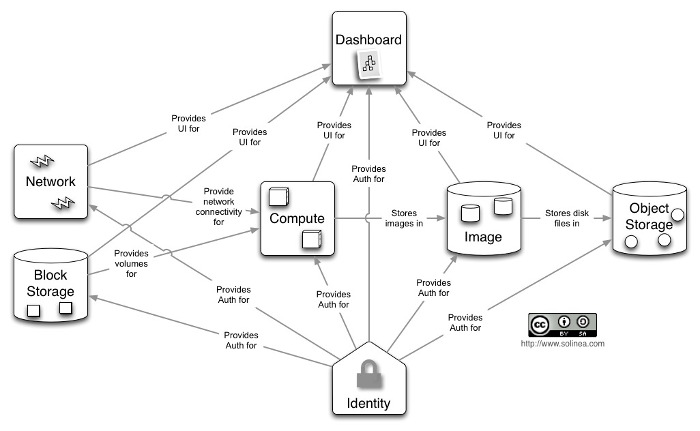
\includegraphics{../Momo/Openstack_diagramme_conceptuel.jpg}
\caption{}
\end{figure}

\subsection{Le Client Python nova}\label{le-client-python-nova}

Le client Python-nova est un client en ligne de commande pour le module
Nova OpenStack , il va nous permmetre de mettre en oeuvre 100\% de l'API
Nova , et aussi la gestion des instances, des images, etc\ldots{}

\subsubsection{Installation de
python-nova}\label{installation-de-python-nova}

Pour installer le plugin python-nova, il faut avoir préalablement
installé python et son système d'installation pip. Pour lancer
l'installation il suffit de taper pip install -U python-novaclient .

\subsubsection{Configuration des variables d'environnement pour
Openstack}\label{configuration-des-variables-denvironnement-pour-openstack}

Pour configurer toutes les variables, Openstack génère un fichier RC
contenant la totalité des variables d'environnement à configurer.

Depuis Cloudwatt il faut aller dans les paramètres \emph{accès et
sécurité} puis \emph{accès API} et enfin télécharger le fichier. En
effet Cloudwatt génère un fichier contenant toutes les variables
d'environnement nécésaire à la configuration de la connexion Openstack.

L'éxécution du fichier se fait grâce à la commande
\texttt{source\ 0750182707\_projet\_tutore\_2017-openrc.sh} et permet la
configuration automatique des variables.

\subsubsection{Liste des instances}\label{liste-des-instances}

La liste des instances créées sont visibles à l'aide de la commande
\texttt{nova\ list}.

\subsection{Création de l'instance}\label{cruxe9ation-de-linstance}

\subsubsection{Génération de la clef
ssh}\label{guxe9nuxe9ration-de-la-clef-ssh}

\texttt{ssh-keygen}

\subsubsection{Intégration clef ssh au keypair
Openstack}\label{intuxe9gration-clef-ssh-au-keypair-openstack}

\texttt{nova\ keypair-add\ -\/-pub-key\ .ssh/id\_rsa.pub\ SSHKEY}

\subsubsection{Choix du flavor}\label{choix-du-flavor}

\texttt{nova\ flavor-list} affiche la liste des flavors disponibles. Une
fois choisi, il faut récuperer son ID qui sera renseigné lors de la
création de l'instance.

\subsubsection{Choix de l'image (système
installé)}\label{choix-de-limage-systuxe8me-installuxe9}

\texttt{nova\ image-list} affiche la liste des images systèmes
disponibles. Une fois choisi, Il faut récuperer son ID qui sera demandé
lors de la génération de l'instance.

\subsubsection{Création de l'instance}\label{cruxe9ation-de-linstance-1}

\texttt{nova\ boot\ -\/-key-name\ SSHKEY\ -\/-flavor\ 16\ -\/-image\ 185e1975-c9c5-4358-909e-5e329808902e\ instance1}

Pour la création de l'instance on retrouve quatre éléments : - le nom du
keypair - l'id du flavor - l'id de l'image - le nom de l'instance


\section{Terraform}\label{terraform}

\subsection{Présenation (Schéma de ou se place dans prod -dans meme
style celui du book crack mais avec ansible en plus (voir xml de
draw.io))}\label{pruxe9senation-schuxe9ma-de-ou-se-place-dans-prod--dans-meme-style-celui-du-book-crack-mais-avec-ansible-en-plus-voir-xml-de-draw.io}

Terraform est un outil développé en Go qui permet la gestion
d'infrastructure à l'aide de recettes. L'objectif de ce logiciel est de
permettre une configuration centralisée, rapide et efficace d'une
infrastructure.

Terraform fonctionne avec des fichiers texte pour configurer les futures
infrastructures. Ces fichiers texte appelé \textbackslash{}og recette
\textbackslash{}fg servent à décrire l'architecture des providers tel
qu'Openstack ou AWS. La configuration se fait dans un fichier
\textbackslash{}og main.tf \textbackslash{}fg qui est écrit en HCL(NOTE:
HashiCorp Configuration Language). La configuration peut aussi être
générée automatiquement par machine avec le format JSON(NOTE).
L'extension du fichier sera alors \textbackslash{}og main.tf.json
\textbackslash{}fg.

Un provider est un service pour le cloud computing, généralement un
IaaS.

Terraform génère un plan d'exécution se basant sur les recettes et
décrivant les étapes qu'il va effectuer. Puis exécute le plan
précédemment défini pour mettre en place l'infrastructure. Terraform
détecte les changements effectué dans les fichiers et créé des nouveaux
plans d'exécution conformément à ses changements.

Terraform permet de gérer les composants de bas niveau comme les IaaS,
le stockage et la mise à niveau, ainsi que des composants hauts niveaux
comme les entrées DNS et les fonctionnalités SaaS.

\subsection{Caractéristiques}\label{caractuxe9ristiques}

\begin{itemize}
\item
  ** Insfrastructure as code : ** L'infrastructure est décrite en
  utilisant une syntaxe de configuration de haut niveau (HCL). Cela
  permet à un data center d'être versionné et traité comme tout autre
  code.
\item
  ** Plan d'exécution : ** Terraform a une étape de \textbackslash{}og
  planification \textbackslash{}fg qui génère un plan d'exécution. Le
  plan d'exécution montre les actions que Terraform effectuera lorsqu'il
  sera lancé. Cela permet d'augmenter la sécurité en évitant d'avoir des
  surprises lorsque Terraform manipule l'infrastructure.
\item
  ** Graphique des ressources : ** Terraform construit un graphique de
  toutes les ressources des infrastructures, et parallélise la création
  et la modification de toutes ces ressources non-dépendantes. Grâce à
  cela, Terraform construit l'infrastructure aussi efficacement que
  possible, et les utilisateurs peuvent avoir un aperçu des dépendances
  de leur infrastructure.
\item
  ** Automatisation des changements : ** Des ensembles complexes de
  changements peuvent être appliqués à une infrastructure avec une
  interaction humaine minimale. Pour se faire Terraform se base sur le
  plan d'exécution et le graphique de ressources mentionnés
  précédemment, évitant ainsi des erreurs humaines possibles.
\end{itemize}

\subsection{Quelques cas d'utilisations (selon la
doc)}\label{quelques-cas-dutilisations-selon-la-doc}

\subsubsection{Self-service Cluster}\label{self-service-cluster}

Dans de grandes organisations, il devient plus attrayant de créer une
infrastructure \textbackslash{}og self-service \textbackslash{}fg,
permettant aux équipes de gérer leur propre infrastructure à l'aide de
l'outillage fourni par l'équipe centrale d'exploitation.

À l'aide de Terraform, la connaissance de la construction de
l'infrastructure et de l'échelle d'un service peut être codifiée dans
une configuration. La configuration de Terraform peut être partagée au
sein d'une organisation permettant aux équipes d'utiliser Terraform
comme un outil pour gérer leurs services sans connaître la
configuration.

\subsubsection{Démos de logiciels}\label{duxe9mos-de-logiciels}

A l'instar de Vagrant qui permet la création d'environnement virtualisé,
les éditeurs de logiciels peuvent fournir une configuration Terraform
pour créer et démarrer une infrastructure de démonstration. Ceci permet
aux utilisateurs finaux de mettre en place rapidement un environnement
de test sur leur propre infrastructure.

\subsubsection{Multi
Cloud-Déploiement}\label{multi-cloud-duxe9ploiement}

Il est souvent attrayant de répandre l'infrastructure sur plusieurs
cloud pour augmenter la tolérance aux pannes. En utilisant une seule
région ou un seul fournisseur cloud , la tolérance aux pannes est
limitée par la disponibilité de ce fournisseur. Avoir un déploiement
multi-cloud permet une meilleure récupération de la perte d'une région
ou tout le fournisseur.

Terraform permet la configuration de plusieurs providers en une seule
configuration. Cela simplifie la gestion et l'orchestration des
providers, en aidant la création d'infrastructures multi-cloud.

\subsection{Syntaxe utilisé}\label{syntaxe-utilisuxe9}

Les configurations de Terraform sont écrites en HashiCorp Configuration
Language (HCL). Ce langage se veut facile à écrire et à lire. L'écriture
des configurations peut aussi se faire en JSON.

\subsubsection{Les bases du langage}\label{les-bases-du-langage}

\emph{Commentaires} - \# sur une seule ligne - /* mon commentaires sur
plusieurs lignes */

\emph{Affectation des valeurs}

\begin{verbatim}
key = value # la valeur peut être une chaîne, un nombre ou un booléen
\end{verbatim}

\emph{Chaînes multilignes} : On utilise
\texttt{\textless{}\textless{}\ -\ EOF} et \texttt{EOF} pour créer des
chaînes multilignes ce qui permet principalement d'intégrer des scripts
dans la configuration.

Il existe également de nombreuses fonctions utilisables avec HCL comme
par exemple la fonction format(format, args, \ldots{}) qui va permettre
de formater une chaîne selon le format que l'on donne.

Les différents blocs se définissent avec des accolades dans le même
principe que des fonctions dans les autres langages connu.
\texttt{language\ ressource\ "nom\_type\_ressource"\ "nomRessource"\ \{\ \ \ \ \ ...\ \}}

\subsection{Fonctionnement}\label{fonctionnement}

Terraform étant développé en Go, il n'a pas besoin d'être installé. Il
suffit de télécharger une archive .zip et de l'extraire. Il est ensuite
possible d'utiliser les commandes associées à Terraform avec
\texttt{./terraform\ ...}. Pour faciliter l'utilisation des commandes,
il est recommandé de copier le fichier dans \emph{/usr/local/} et
d'ajouter ensuite le chemin menant jusqu'au fichier en question dans le
PATH \texttt{PATH=/usr/local/...:\$PATH}.

Terraform peut être composé de plusieurs fichiers de configuration pour
une infrastructure. Dans ce cas, les fichiers sont lus par ordre
alphabétique, mais la priorité reste au fichier \emph{main.tf}.

Les fichiers Terraform se composent de différents type de bloc : le bloc
provider et le bloc ressource. Chacun de ses blocs peut se retrouver
plusieurs fois dans un fichier.

\subsubsection{\texorpdfstring{Bloc
\textbf{\texttt{provider}}}{Bloc provider}}\label{bloc-provider}

C'est la partie configuration du provider avec principalement les accès
pour la connexion à celui-ci. Terraform peut contenir plusieurs blocs
provider. Ce bloc gère le cycle de vie des ressources (create, read,
update, delete).
\texttt{language\ provider\ "openstack"\ \{\ \ \ \ \ user\_name\ \ =\ "admin"\ \ \ \ \ tenant\_name\ =\ "admin"\ \ \ \ \ password\ \ =\ "pwd"\ \ \ \ \ auth\_url\ \ =\ "http://myauthurl:5000/v2.0"\ \}}

Cloudwatt offre la génération d'un fichier .sh avec la totalité des
identifiants est accès pour Openstack. Pour la connection, nous avons pu
ommettre le bloc provider, Terraform se charge de récuperer les
variables environnementales correspondant aux paramètres dont il a
besoin pour retrouver le provider.

\subsubsection{\texorpdfstring{Bloc
\textbf{\texttt{resource}}}{Bloc resource}}\label{bloc-resource}

Partie permettant la gestion des ressources (composants physiques et
logiciels) qui existent dans l'infrastructure. Le nom d'une ressource se
compose du nom du provider puis du nom de la ressource en un bloc et
enfin un nom pour cette ressource terraform qui sera utilisé uniquement
par terraform.
\texttt{language\ resource\ "openstack\_compute\_instance\_v2"\ "nomTerraform"\ \{\ \}}

\subsubsection{Variables}\label{variables}

Les variables peuvent être enregistrées dans un fichier
\textbackslash{}og variables.tf \textbackslash{}fg ou \textbackslash{}og
.tfvars \textbackslash{}fg. Pour appliquer des variables enregistrées
sous cette dernière extension, il faut lancer la commande suivante
\texttt{terraform\ apply\ -var-file=truc.tfvars}. Les variable sont
généralement utilisé dans les fichiers sous la forme suivante
\texttt{\$\{var.nomVar\}}.

\subsubsection{Modules}\label{modules}

Il est possible d'intégrer des modules à Terraform. Terraform se charge
du téléchargement et de l'intégration des modules. L'appel d'un module
se fait de la même manière qu'une ressource mais avec le mot clef
\emph{module}. La source est ensuite indiquée dans une variable. La
source peut provenir d'un dépot github, d'une archive (de multiples
format sont compris comme tar.gz, zip, bz2\ldots{}), d'un dossier
local\ldots{} Concrétement un module Teraform est un dossier contenant
des fichiers \emph{.tf} qui ont besoin d'être utilisé plusieurs fois.
Pour régler ce problème de copie multiple du code, il est possible
d'utiliser ce dossier en-tant que module et ainsi avoir un code plus
clair.

\subsubsection{Plugins}\label{plugins}

Terraform a été crée avec la possibilité d'importer des plugins. Pour
installer un plugin, il faut récuperer le code du plugin, et créer un
fichier \emph{\textasciitilde{}/.terraformrc} contenant un bloc
providers avec une variable indiquant le chemin jusqu'au dossier du
plugin. L'utilisation du plugin se fait apres dans le fichier .tf de
l'insfrastructureet s'utilise comme un bloc ressource normal en suivant
la syntaxe définie dans la documentation du plugin en question.

\subsubsection{Les commandes}\label{les-commandes}

\begin{itemize}
\tightlist
\item
  \texttt{terraform\ plan} -- génère un plan d'action de la
  configuration. Le plan inclu toutes les actions faites et montre les
  modifications que va effectuer Terraform.
\item
  \texttt{terraform\ plan\ -destroy\ -out=destroy.tf} -- génère un plan
  d'action qui à pour objectif de détruire tous le projet défini pas les
  fichiers de configuration. Le résultat est enregistré dans un fichier
  pour ensuite être appliqué avec \texttt{terraform\ apply\ destroy.tf}.
\item
  \texttt{terraform\ destroy} -- détruit l'infrastructure généré par
  Terraform avec le compte importé (idendique à la technique du dessus).
\item
  \texttt{terraform\ apply} -- applique le code Terraform en générant ce
  que \texttt{terraform\ plan} à montré précédement
\item
  \texttt{terraform\ graph} -- permet la visualisation du plan en images
\item
  \texttt{terraform\ show} -- montre les infrastructures en place
\end{itemize}

\subsection{Configurations
effectuées}\label{configurations-effectuuxe9es}

\subsubsection{Keypair}\label{keypair}

Une des premières configurations effectuées fut l'ajout de clef ssh pour
le projet. Cet ajout avait pour objectif de nous permettre de nous
connecter en ssh avec les instances créées.
\texttt{language\ resource\ "openstack\_compute\_keypair\_v2"\ "my\_keypair"\ \{\ \ \ name\ =\ "my\_keypair"\ \ \ public\_key\ =\ "\$\{var.keypair\}"\ \}}
Terraform prend en paramètre pour cette resource un nom et la clef
publique à ajouter. Cette clef ssh est requise lors de la création
d'instance. En effet celles-ci prennent en paramètre une keypair -
\texttt{key\_pair\ =\ "\$\{openstack\_compute\_keypair\_v2.my\_keypair.name\}"}
- pour permettre la connection ssh à l'instance en question. Cependant
une seule keypair peut être intégrée dans la ressource \emph{instance}.
Pour avoir tous accès en ssh aux instances, nous nous sommes paratagés
la clef privé créée spécialement pour le projet et n'ayant pas de
passphrase pour permettre à ansible de se connecter ensuite.

\subsubsection{Instances}\label{instances}

Les instances sont la plus grande partie de la configuration, elles
correspondent aux réseaux privés virtuels (vps) qui vont être créées.
```language resource ``openstack\_compute\_instance\_v2'' ``vps'' \{
count = 3 name = ``vps-test-\$\{(count.index)+1\}'' image\_id =
``185e1975-c9c5-4358-909e-5e329808902e'' flavor\_id = ``16'' key\_pair =
``\$\{openstack\_compute\_keypair\_v2.my\_keypair.name\}''
security\_groups =
{[}``\$\{openstack\_compute\_secgroup\_v2.terraform.id\}''{]}
floating\_ip =
``\$\{element(openstack\_compute\_floatingip\_v2.terraform.*.address,
count.index+1)\}"

network \{ name =
``\$\{openstack\_networking\_network\_v2.network\_1.name\}''
fixed\_ip\_v4 = ``192.168.0.1\$\{(count.index)+1\}'' \} \}
``\texttt{Une\ instance\ peut\ être\ créée\ dans\ une\ configuration\ unique,\ mais\ il\ est\ aussi\ possible\ d\textquotesingle{}en\ générer\ plusieurs\ automatiquement\ avec\ une\ seule\ ressource\ associée\ grâce\ au\ paramètre}count\texttt{.\ La\ création\ des\ insantances\ se\ fait\ donc\ en\ partant\ de\ zéro.\ Avec}count.index`
nous pouvons récuperer l'index actuel de la boucle générée par
tarraform. Chaque instance est ratachée à un ou plusieurs réseaux selon
les besoins. Pour notre proof of concept, nous avons utilisé un seul
réseau. Pour connecter les instances au réseau, il faut écrire un bloc
\emph{network} comme ci-dessus.

\subsubsection{Security group}\label{security-group}

Le security group permet d'autoriser les transmissions sur certain port.
Un security group fonctionne sur le même principe qu'un firewall. Il est
conposé de règles \emph{rule}. Une règle est définit pour un port. Nous
avons crés un security group nommé \textbackslash{}og terraform
\textbackslash{}fg composé d'une seule règle permettant la connection
ssh (port 22).
\texttt{language\ resource\ "openstack\_compute\_secgroup\_v2"\ "terraform"\ \{\ \ \ name\ \ \ \ \ \ \ \ =\ "terraform"\ \ \ description\ =\ "security\ group"\ \ \ rule\ \{\ \ \ \ \ from\_port\ \ \ =\ 22\ \ \ \ \ to\_port\ \ \ \ \ =\ 22\ \ \ \ \ ip\_protocol\ =\ "tcp"\ \ \ \ \ cidr\ \ \ \ \ \ \ \ =\ "0.0.0.0/0"\ \ \ \}\ \}}

\subsubsection{Ip flotantes}\label{ip-flotantes}

Les ip flotantes permettent aux instances d'avoir une ip publique.
Permettant ainsi de pouvoir accéder en ssh aux instances. Terraform
offre la posibilité de générer automatiquement les adresses ip en les
piochant dans un pool public d'adresses. Cependant l'utiisation
d'ansible requière la connaissance des adresses ip flottantes attribuée
aux machines. Pour ce faire plusieurs solutions s'offraient à nous. - La
première est l'importation des adresses ip avec
\texttt{terraform\ import}. Cependant Terraform ne permet pas la
création de boucle, seule la variable \emph{count} est utilisable. Le
changement de nom de la ressource importée est impossible avec ce
système de boucle. L'importation avec terraform fonctionne de la manière
suivante : La ressource est importé avec la commande, mais pour être
utilisable elle doit avoir une ressource créée dans le fichier .tf.
L'importation d'une multitude d'adresses ip entrainaient la création du
même nombre de ressources le tout créé à la main. La tâche devenaient
vite fastidieuse. - La seconde solution est la création d'une liste
contenant les adresses ip floatantes créées depuis l'interface web de
l'hébergeur. L'appel de l'adresse se fait depuis la ressource instance
de terraform qui vas récuperer une adresse dans la liste.

```language

\section{Fichier variables.tf}\label{fichier-variables.tf}

variable ``id\_ip\_flottante'' \{ default =
{[}``84.39.49.19'',``84.39.46.157'',``84.39.44.165'',``84.39.41.206''{]}
\}

\section{Fichier main.tf}\label{fichier-main.tf}

resource ``openstack\_compute\_instance\_v2'' ``vps'' \{ floating\_ip =
``\$\{var.id\_ip\_flottante{[}(count.index)+1{]}\}'' \} ``` Nous avons
donc choisit cette dernière pour mettre en place le système d'ip
flotantes dans notre infrastructure terraform.

\subsubsection{Réseau, sous-réseau et
routeur}\label{ruxe9seau-sous-ruxe9seau-et-routeur}

Terraform permettant de créer toute une infrastructure, nous nous sommes
aussi penchés sur la création du réseau, de ses sous-réseaux et du
routeur nous permettant un accès au monde extérieur.

\paragraph{Réseau et sous-réseau}\label{ruxe9seau-et-sous-ruxe9seau}

Pour être utilisable, les instances doivent être connectées à un réseau.
Terraform offre la possibilité de crée rapidement et facilement un
réseau ainsi que les sous-réseaux et port utile à celui-ci. Les
instances sont donc configurées pour être intégrées à ce réseau et
obtenir une adresse ip dans ce dernier. ```language resource
``openstack\_networking\_network\_v2'' ``network\_1'' \{ name =
``resTerraform'' admin\_state\_up = ``true'' \}

\section{Sous-réseau}\label{sous-ruxe9seau}

resource ``openstack\_networking\_subnet\_v2'' ``subnet\_2'' \{ name =
``SousRes\_2'' network\_id =
``\$\{openstack\_networking\_network\_v2.network\_1.id\}'' cidr =
``192.168.0.0/24'' ip\_version = 4 \}

\section{Port du sous-réseau}\label{port-du-sous-ruxe9seau}

resource ``openstack\_networking\_port\_v2'' ``port\_1'' \{ name =
``port\_1'' network\_id =
``\$\{openstack\_networking\_network\_v2.network\_1.id\}''
admin\_state\_up = ``true'' \} ```

\paragraph{Routeur}\label{routeur}

Pour que l'infrastructure créée soit opérationelle, il faut lui
autoriser un accès à l'extérieur du réseau. Pour se faire nous passons
par un routeur qui est lui même composé d'une interface le relinant à un
des réseau crée précedement.
\texttt{language\ resource\ "openstack\_networking\_router\_v2"\ "router\_1"\ \{\ \ \ name\ =\ "routerTerraform"\ \ \ admin\_state\_up\ =\ "true"\ \ \ external\_gateway\ =\ "6ea98324-0f14-49f6-97c0-885d1b8dc517"\ \}}

\begin{figure}
\centering
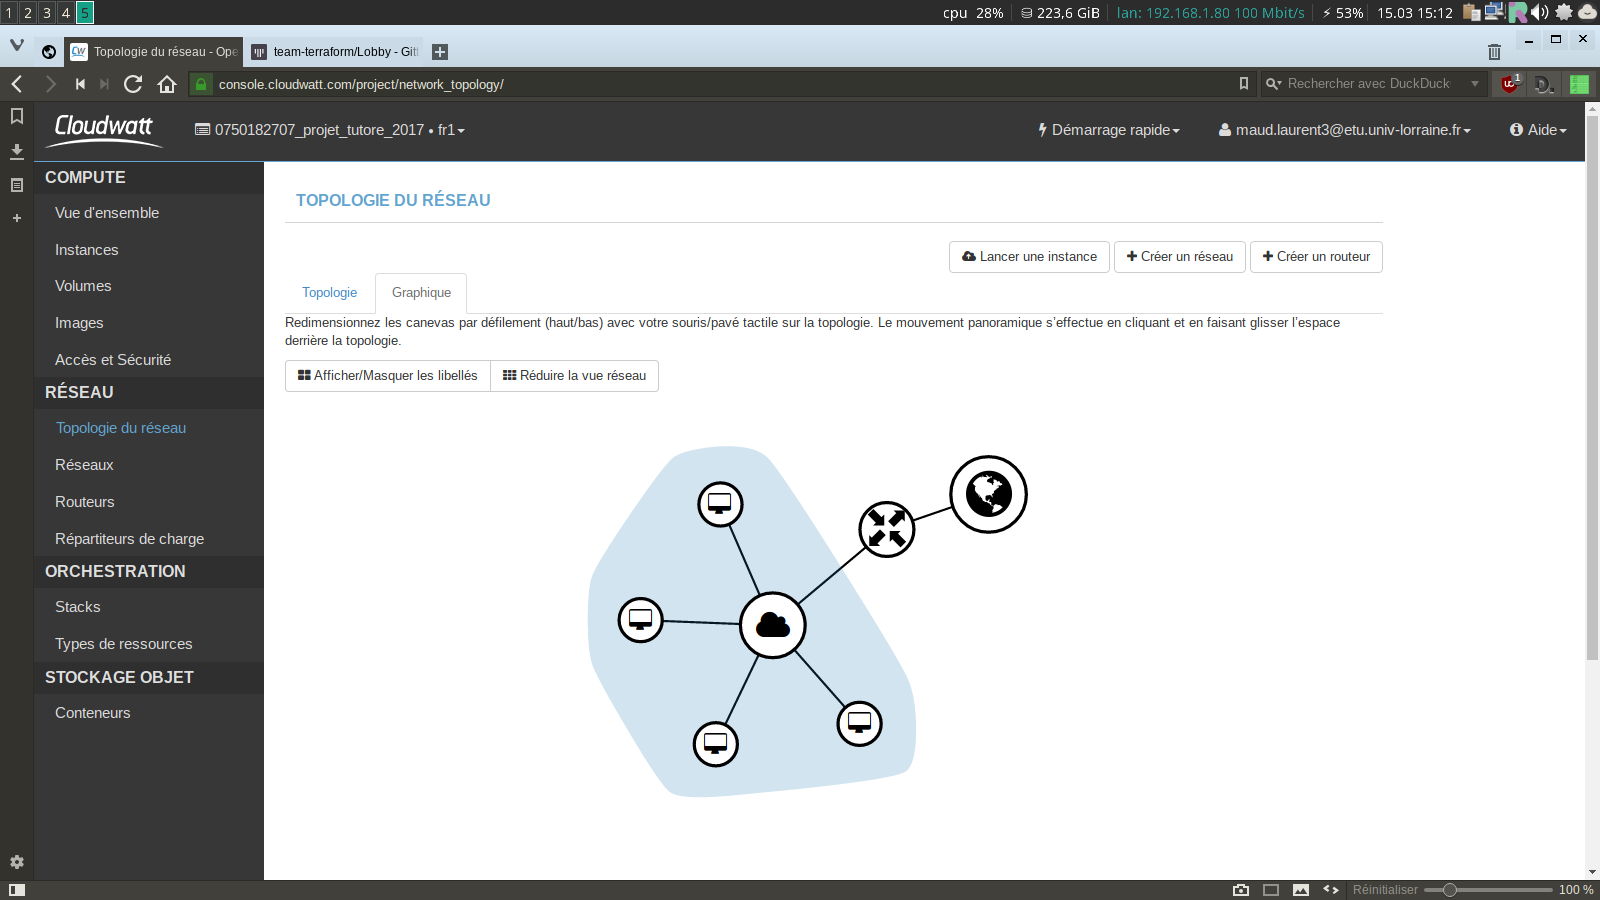
\includegraphics{./reseau.png}
\caption{reseau.png}
\end{figure}

\section{Provisionnement}\label{provisionnement}

Terraform permet aussi le provisionnement de ses instances avec
différents provisionners comme chef, puppet ou encore ansible. Cependant
Terraform n'offre un service que pour Chef mais permet d'éxécuter
différentes commandes automatiquement depuis la machine lancant
\texttt{terraform\ apply} avec le provisionner \texttt{local\_exec} ou
depuis la machine générée avec Terraform grâce au provisionner
\texttt{remote\_exec}. Celui-ci se compléte avec le bloc
\texttt{connection} effectuant une connexion ssh avec les identifiants
désiré. Ces dernières se mettant dans les instances. Les ressources de
type \texttt{null-ressource} permettent d'executer des commandes après
la création des certaines ressources. Grâce à cela, il est possible de
lancer ansible automatiquement à la fin de la création des vps.

\section{Ansible}\label{ansible}

\subsection{Présentation}\label{pruxe9sentation}

\subsection{Utilisation, Fonctionnement,
syntaxe}\label{utilisation-fonctionnement-syntaxe}

\subsection{Intégration à
Terraform}\label{intuxe9gration-uxe0-terraform}

\subsection{Configuration effectuée (pk on l'a fait, surtout expliqué
pour les clef
ssh)}\label{configuration-effectuuxe9e-pk-on-la-fait-surtout-expliquuxe9-pour-les-clef-ssh}

\section{Répartition des tâches au seins du
groupe}\label{ruxe9partition-des-tuxe2ches-au-seins-du-groupe}

Le projet se tenait sur une seule technologie qui est Terraform. La
répartition des tâches c'est donc faite par rapport aux différentes
parties que nous avons du créer pour faire fonctionner notre
infrastructure. (TODO: Diagramme de GANTT ? ou truc semblable ?)

\section{Avant TerraForm}\label{avant-terraform}

\subsection{AWS CloudFormation}\label{aws-cloudformation}

CloudFormation fournit par Amazon Web Service permet de créer et de
gérer un ensemble de ressources qui sont liées, de les ordonner, les
mettre en service et les actualiser en mode ordonnée. Il permait d'avoir
aussi une infrastructure as code avec des simples fichiers textes au
format JSON ou YAML. Il fonctionne uniquement avec AWS mais le
fonctionnement resemble à Terraform. Il permet de créer un modèle qui
décrit toutes les ressources AWS que l'on veut (telles que des instances
Amazon EC2 ou des instances de base de données Amazon RDS). De plus AWS
CloudFormation s'occupe de leur mise en service et de leur
configuration. AWS CloudFormation a des modéles d'exemples déjà crée qui
peuvent etre utilisés. Il est aussi possible de créer des modèles
personalisés.

\subsection{Heat}\label{heat}

Heat est un module de la partie orchestraction de OpenStack. La mission
du programme OpenStack Orchestration est de créer un service accessible
pour gérer l'ensemble du cycle de vie des infrastructures et des
applications dans le cloud OpenStack. Heat fournit une orchestration à
base de modèle pour décrire une application cloud. En s'exécutant
OpenStack appels différentes API pour générer l'exécution d'applications
cloud. Un template Heat décrit l'infrastructure pour une application
cloud dans des fichiers textes qui sont lisibles et modifiables par les
humains, et peut être géré par des outils de contrôle de version. Le
logiciel intègre d'autres composants d'OpenStack. Les modèles permettent
la création de la plupart des types de ressources OpenStack tels que les
instances, ip flottantes, des volumes, des groupes de sécurité, les
utilisateurs, etc. Ainsi que certaines fonctionnalités plus avancées
telles que la haute disponibilité. Heat gère principalement
l'infrastructure, mais les templates intègrent aussi des outils de
gestion de configuration logiciel tels que Puppet et Ansible.

\section{TerraForm vs les autres
logiciels}\label{terraform-vs-les-autres-logiciels}

Les outils comme CloudFormation, Heat, etc\ldots{} permettent à une
infrastructure d'être codifiés dans un fichier de configuration. Les
fichiers de configuration permettent à l'infrastructure d'être
élastiquement créé, modifiée et détruite. Terraform est inspiré par les
problèmes qu'ils résolvent.

Terraform utilise de la même façon des fichiers de configuration pour
détailler la configuration de l'infrastructure, mais il va plus loin par
le diagnostique ainsi que la permission de fournisseurs multiples et des
services combiné et composé. Par exemple, Terraform peut être utilisé
pour orchestrer un AWS et un groupe OpenStack simultanément, en
permettant des fournisseurs du 3ème parti comme CloudFlare et DNSIMPLE
d'être intégré pour fournir des services de DNS et CDN. Ceci permet à
Terraform de représenter et gérer l'infrastructure entière avec ses
services de soutien. Au lieu de seulement le sous-ensemble qui existe
dans un fournisseur seul. Il fournit une syntaxe unifiée, au lieu
d'exiger que des opérateurs utilisent des outils indépendants et
non-interopérables pour chaque plate-forme et service.

Terraform sépare également la phase de planification de la phase
d'exécution, en utilisant le concept d'un plan d'exécution. En exécutant
terraform plan, l'état actuel est actualisé et la configuration est
consulté pour générer un plan d'action. Le plan comprend toutes les
actions à entreprendre. Quelles ressources seront créés, détruites ou
modifiées ? Terraform génère un plan d'exécution décrivant ce qu'il va
faire pour atteindre l'état désiré. En utilisant terraform graph, le
plan peut être visualisé pour montrer les commandes qui vont être
executées par celui-ci . Une fois que le plan est capturé, la phase
d'exécution peut être limitée aux seules actions du plan. D'autres
outils combinent les phases de planification et d'exécution, ce qui
signifie que terraform montre les effets de changement qui va se
produire sur l'infrastructure, qui devient rapidement insoluble dans les
grandes infrastructures. Terraform permet aux opérateurs d'appliquer des
changements avec confiance, car ils savent exactement ce qui se passera
au préalable.

\section{Conclusion}\label{conclusion}

TerraForm est un outils formidable permmetant de deployer des
infrastructures de maniere simple et efficace. Il fournit une syntaxe
simple et unifiée permettant de gérer presque toutes les ressources sans
apprendre de nouveaux outils. En outre, Terraform est un outil open
source. En plus de HashiCorp, la communauté autour de Terraform
contribue à étendre ses fonctionnalités, corriger les bugs et documenter
de nouveaux cas d'utilisation. Terraform aide à résoudre un problème qui
existe dans chaque organisation et fournit un standard qui peut être
adoptée pour éviter de réinventer la roue entre et au sein des
organisations.

\end{document}
